Esto modifica la velocidad de los ciclos de la onda.

\[\boxed{
  f(x)=\sin(fx)
}\]

\begin{tikzpicture}
  \begin{axis}[
    xmin=0,xmax=2.2*pi,
    ymin=-1.2,ymax=1.2,
    axis lines=middle,
    xtick={0},
    xtick={pi/2,pi,3*pi/2,2*pi},
    xticklabels={
      $\dfrac{\pi}{2}$,
      $\pi$,
      $\dfrac{3}{2}\pi$,
      $2\pi$
    },
    xticklabel style={anchor=south west},
    ytick={-1,1},yticklabels={$-1$,$1$}
    ]

    \addplot[color=red,samples=100,domain=0:2*pi,thick]{sin(deg(x))};

    \addplot[color=green,samples=100,domain=0:2*pi,thick]{sin(2*deg(x))};

    \addplot[color=blue,samples=100,domain=0:2*pi,thick]{sin(3*deg(x))};

    \legend{$\sin(x)$, $\sin(2x)$, $\sin(3x)$}
  \end{axis}
\end{tikzpicture}
